%\documentclass[11pt,a4paper]{article}
%\usepackage{polski}
%\usepackage[utf8]{inputenc}
%\usepackage{graphicx}

\title{Projektowanie algorytmów i metod sztucznej inteligencji. Laboratorium  9 - Sprawozdanie}
\author{Wojciech Makuch}
\date{}

%\begin{document}
	\maketitle
	\section{Zadanie}\label{sec:Zadanie}
	Implementacja grafu oraz zbadanie złożoności obliczeniowej algorytmów przeszukiwania w głąb(ang. \textsl{Depth-first search, DFS}) oraz przeszukiwania  wszerz(ang. \textsl{breadth-first search, BFS}).
	
	\section{Wstep}\label{sec:Wstep}
	Graf – abstrakcyjna struktura danych. Jest zbudowana z wierzchołków i krawędzi. Wierzchołki grafu mogą być numerowane i czasem stanowią reprezentację jakichś obiektów, natomiast krawędzie mogą wówczas obrazować relacje między takimi obiektami. Wierzchołki należące do krawędzi nazywane są jej końcami. Krawędzie mogą mieć wyznaczony kierunek, a graf zawierający takie krawędzie nazywany jest grafem skierowanym. Krawędź grafu może posiadać wagę, to znaczy przypisaną liczbę, która określa, na przykład, odległość między wierzchołkami.
	\\
	\\
	Przeszukiwanie w głąb - polega na badaniu wszystkich krawędzi wychodzących z podanego wierzchołka. Teoretyczna złożoność czasowa przeszukiwania w głąb wynosi $O(|V|+|E|)$, gdzie V-ilość wierzchołków, E – ilość krawędzi. Teoretyczna złożoność pamięciowa wynosi $O(h)$, gdzie h – długość najdłuższej prostej ścieżki.
	\\
	\\
	Przeszukiwanie wszerz - przechodzenie grafu rozpoczyna się od zadanego wierzchołka i polega na odwiedzeniu wszystkich osiągalnych z niego wierzchołków. Teoretyczna złożoność czasowa wynosi również $O(|V|+|E|)$. Złożoność pamięciowa w tym przypadku też wynosi $O(|V|+|E|)$.
	
	\section{Graf - implementacja}\label{sec:Graf - implementacja}
	Utworzono klasy przechowujące elementy grafu takie krawędzie i wierzchołki oraz klasę nadrzędną, która łączy je w jeden graf. Informacja o połączeniu wierzchołków i krawędzi jest zapisywana w macierzy sąsiedztwa. Do zaalokowania pamięci niezbędne jest wcześniejsze podanie rozmiaru. Głowna funkcja programu zawiera menu użytkownika pozwalające testować poprawność programu oraz testować złożoność obliczeniową badanych algorytmów.
	
	\section{Zlozonosci obliczeniowe usyskane}\label{sec:Zlozonosci obliczeniowe usyskane}
	Na rys 1. pokazano uzyskane wyniki badania złożoności obliczeniowej dla algorytmu DFS, natomiast to samo dla algorytmu BFS przedstawiono na rys 2. Z obydwu rysunków wynika, że złożoność czasowa jest w przybliżeniu stała i oscyluje w granicy wartości 1000.  Z praktycznego punktu widzenia jest to złożoność zgodna z teoretyczną ponieważ zaimplementowana w programie metoda tworzenia losowych grafów tworzy również losowe krawędzie, przez co w większości wypadków nie wszystkie wierzchołki są połączone z grafem - tworzy się graf niepołączony/niespójny. W efekcie ilość krawędzi jest dużo mniejsza.
	\begin{figure}[h]
	\centering
	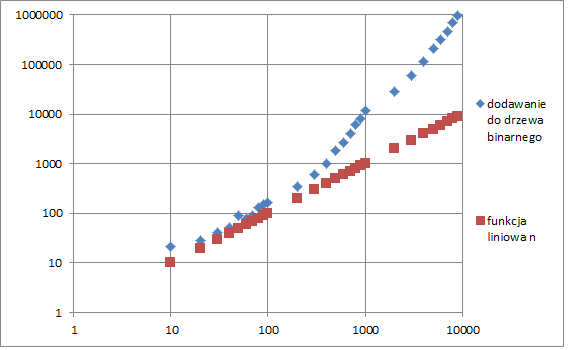
\includegraphics[scale=0.9]{1.png}
	\caption{Dodawanie do drzewa binarnego.}
	\label{fig:1}
	\end{figure}
	\begin{figure}
	\centering
	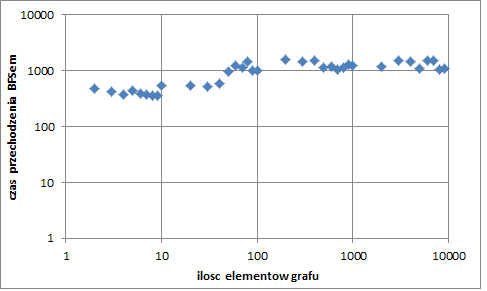
\includegraphics[scale=0.90]{2.png}
	\caption{Prszeszukiwanie drzewa binarnego.}
	\label{fig:2}
	\end{figure}

	\section{Komentarz}\label{sec:Komentarz}
	Do utworzenia dokumentacji wykorzystano system Doxygen. Funkcja pomiaru czasu dla systemu Windows pobrana ze strony dr. J. Mierzwy. Program skompilowano w środowisku Code::Blocks. Do stworzenia wykresu posłużono się pakietem MS Excel, sprawozdanie napisano używając systemu \LaTeX.
	
\begin{thebibliography}{99}
	\bibitem{1} http://pl.wikipedia.org/wiki/Przeszukiwanie\_w\_glab
	\bibitem{2} http://pl.wikipedia.org/wiki/Przeszukiwanie\_wszerz
\end{thebibliography}

\end{document}
